\documentclass[tikz,border=6pt]{standalone}
\usetikzlibrary{arrows.meta,positioning,calc,fit,matrix}
\makeatletter
\AtBeginDocument{\global\let\pgf@selectfontorig\relax}
\makeatother

\tikzset{
  nodebox/.style={draw=#1, rounded corners=4pt, very thick, fill=gray!4,
    minimum width=12mm, minimum height=8mm, align=center, inner sep=2pt},
  nodebox/.default=black,
  initial/.style={-Latex, very thick},
  edge/.style={-Latex, very thick, shorten >=3pt, shorten <=3pt},
  labelbox/.style={inner sep=4pt},
  aptxt/.style={text=gray!65!black, anchor=north west}
}

\newcommand{\initarrow}[3]{\draw[initial] #1 -- node[labelbox,auto] {\scriptsize #2} (#3);}
\begin{document}
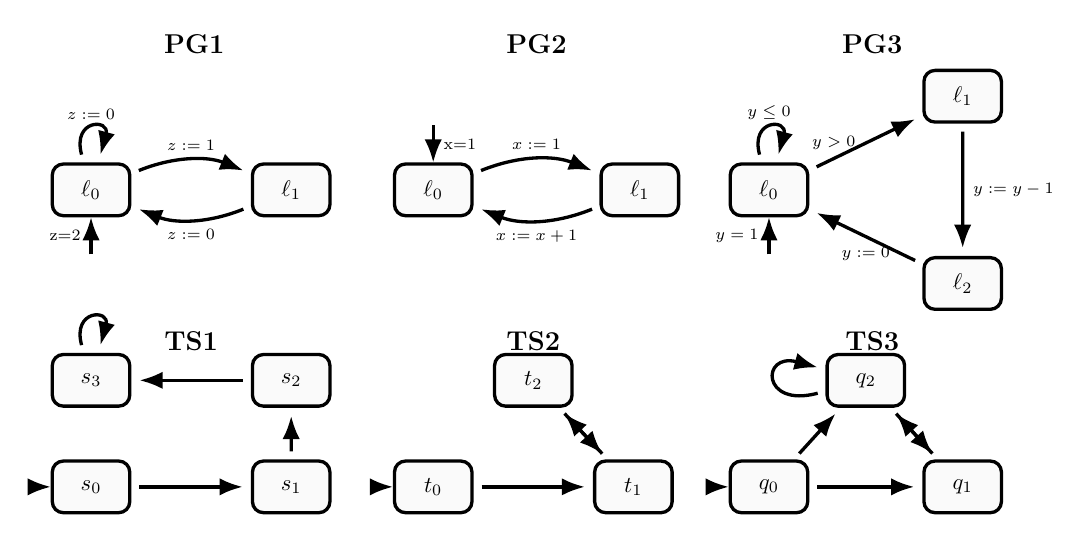
\begin{tikzpicture}[scale=.82, transform shape]
  \begin{scope}[shift={(0,0)}]
    \node at (1.55,2.25) {\bfseries\large TS1};
    \node[nodebox] (s0) at (0,0) {$s_0$};
    \node[nodebox] (s1) at (3.1,0) {$s_1$};
    \node[nodebox] (s2) at (3.1,1.65) {$s_2$};
    \node[nodebox] (s3) at (0,1.65) {$s_3$};
    \initarrow{(-.85,0)}{}{s0.west}
    \draw[edge] (s0) -- (s1);
    \draw[edge] (s1) -- (s2);
    \draw[edge] (s2) -- (s3);
    \draw[edge,loop above,looseness=8] (s3) to (s3);
  \end{scope}

  \begin{scope}[shift={(5.3,0)}]
    \node at (1.55,2.25) {\bfseries\large TS2};
    \node[nodebox] (t0) at (0,0) {$t_0$};
    \node[nodebox] (t1) at (3.1,0) {$t_1$};
    \node[nodebox] (t2) at (1.55,1.65) {$t_2$};
    \initarrow{(-.85,0)}{}{t0.west}
    \draw[edge] (t0) -- (t1);
    \draw[edge] (t1) -- (t2);
    \draw[edge] (t2) -- (t1);
  \end{scope}

  \begin{scope}[shift={(10.5,0)}]
    \node at (1.6,2.25) {\bfseries\large TS3};
    \node[nodebox] (q0) at (0,0) {$q_0$};
    \node[nodebox] (q1) at (3,0) {$q_1$};
    \node[nodebox] (q2) at (1.5,1.65) {$q_2$};
    \initarrow{(-.85,0)}{}{q0.west}
    \draw[edge] (q0) -- (q1);
    \draw[edge] (q1) -- (q2);
    \draw[edge] (q2) -- (q1);
    \draw[edge] (q0) -- (q2);
    \draw[edge,loop left,looseness=8] (q2) to (q2);
  \end{scope}

  \begin{scope}[shift={(0,4.6)}]
    \node at (1.6,2.25) {\bfseries\large PG1};
    \node[nodebox] (l0) at (0,0) {$\ell_0$};
    \node[nodebox] (l1) at (3.1,0) {$\ell_1$};
    \initarrow{(0,-1)}{z=2}{l0.south}
    \draw[edge,bend left=22] (l0) to node[labelbox,above] {\scriptsize $z:=1$} (l1);
    \draw[edge,bend left=22] (l1) to node[labelbox,below] {\scriptsize $z:=0$} (l0);
    \draw[edge,loop above,looseness=8] (l0) to node[labelbox,above] {\scriptsize $z:=0$} (l0);
  \end{scope}

  \begin{scope}[shift={(5.3,4.6)}]
    \node at (1.6,2.25) {\bfseries\large PG2};
    \node[nodebox] (l0) at (0,0) {$\ell_0$};
    \node[nodebox] (l1) at (3.2,0) {$\ell_1$};
    \initarrow{(0,1)}{x=1}{l0.north}
    \draw[edge,bend left=22] (l0) to node[labelbox,above] {\scriptsize $x:=1$} (l1);
    \draw[edge,bend left=22] (l1) to node[labelbox,below] {\scriptsize $x:=x+1$} (l0);
  \end{scope}

  \begin{scope}[shift={(10.5,4.6)}] 
    \node at (1.6,2.25) {\bfseries\large PG3};
    \node[nodebox] (l0) at (0,0) {$\ell_0$};
    \node[nodebox] (l1) at (3,1.45) {$\ell_1$};
    \node[nodebox] (l2) at (3,-1.45) {$\ell_2$};
    \initarrow{(0,-1)}{$y=1$}{l0.south}
    \draw[edge] (l0) -- node[labelbox,left] {\scriptsize $y>0$} (l1);
    \draw[edge] (l1) -- node[labelbox,right] {\scriptsize $y:=y-1$} (l2);
    \draw[edge] (l2) -- node[labelbox,below] {\scriptsize $y:=0$} (l0);
    \draw[edge,loop above,looseness=8] (l0) to node[labelbox,above] {\scriptsize $y\le0$} (l0);
  \end{scope}
\end{tikzpicture}
\end{document}
  
